\section{Choosing a Step Size for Policy Gradients}
\begin{frame}{Choosing a Step Size for Policy Gradients}
\begin{itemize}
    \item But, the problem is more than step size
    \item Distance in parameter space $\ne$ distance in policy space!
    \item Small changes in the policy parameters can unexpectedly lead to big changes in the policy.
    \pause
    \item Consider a family of policies with parametrization:
    \[ \pi_\theta(a) = \begin{cases} 
          \sigma(\theta) & a = 1 \\
          1 - \sigma(\theta) & a=2 
       \end{cases}
    \]
    \pause
    
\end{itemize}
\begin{figure}
\centering
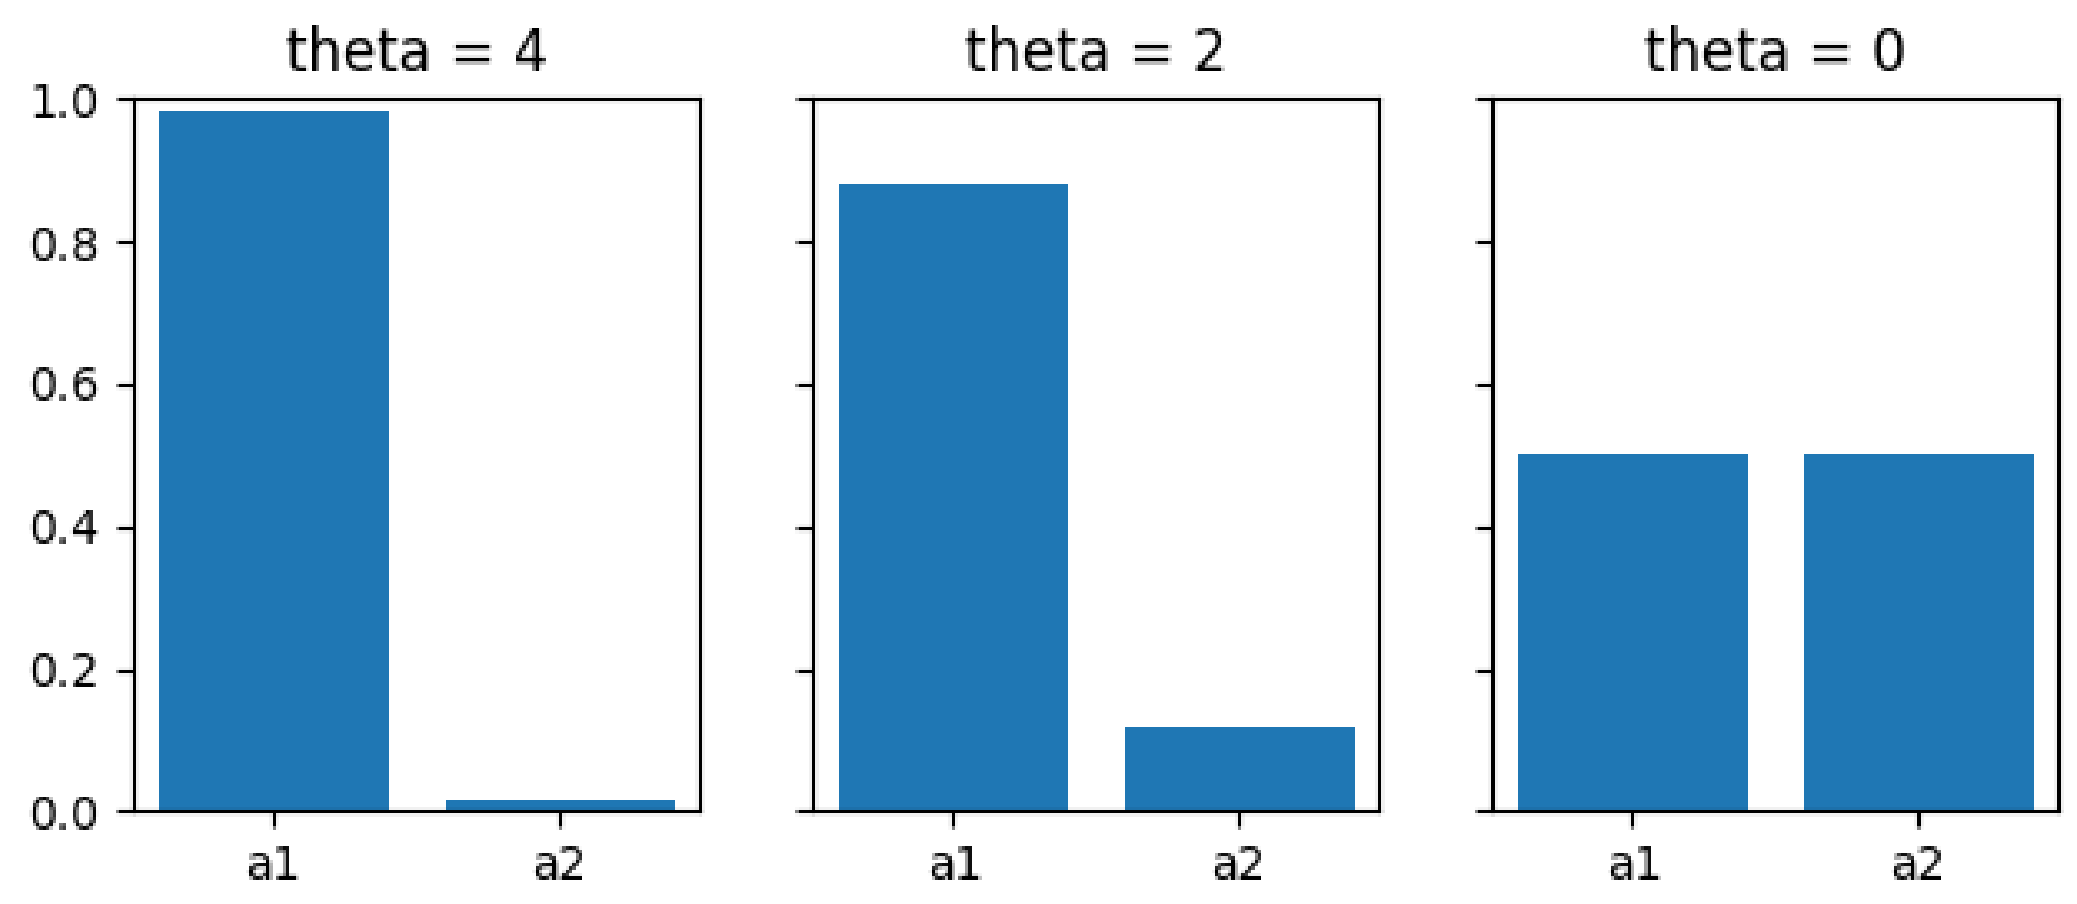
\includegraphics[width=0.9\textwidth,height=0.4\textheight,keepaspectratio]{images/policy-search/step_2.png}
\end{figure}
    
\end{frame}